
\documentclass[usletter, 10pt, conference]{ieeeconf}
\newcommand{\mbm}[1]{\mbox{\boldmath $#1$}}
\newcommand{\norm}[1]{\lVert#1\rVert}
\newcommand{\superscript}[1]{\ensuremath{^{\textrm{#1}}}}
\newcommand\blfootnote[1]{%
  \begingroup
  \renewcommand\thefootnote{}\footnote{#1}%
  \addtocounter{footnote}{-1}%
  \endgroup
}
\usepackage{url}

\usepackage[ruled]{algorithm2e}
\usepackage{subfigure}
\usepackage{graphicx,color,psfrag}
\usepackage{amsmath}
\usepackage{amsfonts}
\usepackage{amssymb}
\usepackage{bigdelim}
\usepackage{dsfont}
\usepackage{color, soul}
%\usepackage[section]{placeins}
%\usepackage{graphicx}
%\usepackage{caption}
%\usepackage{subcaption}

\overrideIEEEmargins
\title{The Autonomous Picking \& Palletizing (APPLE) Robot:\\ A Research Platform for
  Intralogistics Applications} 

% Multiple authors
\author{ \authorblockN{Robert Krug\superscript{*}, Todor Stoyanov\superscript{*}, Vinicio
    Tincani\superscript{\ddag}, Henrik Andreasson\superscript{*},\\ Rafael Mosberger\superscript{*},
    Gualtiero Fantoni\superscript{\ddag}, Achim J. Lilienthal\superscript{*} and Antonio
    Bicchi\superscript{\ddag}}
 %\authorblockA{\superscript{*}AASS Research Center, {\"O}rebro University, Sweden}
}

\begin{document}
\maketitle
\thispagestyle{empty}
\pagestyle{empty}
%
\blfootnote{\hspace{-4.5mm} \superscript{*} AASS Research Center; {\"O}rebro University; Studentgatan 1, 70182 {\"O}rebro, Sweden.\\
  \superscript{\ddag} Interdepart. Research Center ``E. Piaggio''; University of Pisa, Via Diotisalvi 2, 56100 Pisa, Italy.}
%
\begin{abstract}
  In this work we present a research platform for fully autonomous commissioning tasks in
  intralogistics settings. The robot comprises a nonholonomic mobile base and a manipulation system
  consisting of a lightweight arm and an under-actuated gripper with active surfaces. The platform
  is capable of autonomously picking up pallets and loading them with unstructured goods in a manner
  which is safe for human workers sharing the environment. Target object handling is accomplished
  via a novel, redundant grasp representation which allows for redundancy in the gripper pose
  placement. This redundancy is exploited by an optimization-based control system which generates
  reactive manipulator motions on-the-fly without the delays occurring in sense-plan-act
  architectures.
\end{abstract}
%
\section{Introduction}
\label{sec:intro}
%
The increasing need for fast and flexible commissioning ($i.\,e.,$ order picking and collection of
unstructured goods from storage compartments in warehouses) in logistic scenarios has created
substantial interest for autonomous robotic solutions. One of the main arguments for automating this
task is that the dull and strenuous nature of commissioning could cause mental and physical illness
in human workers. As a result, the determination within the logistics sector to invest in this area
is high and substantial efforts are made for the humanization of workstations~\cite{Eche08}.

There exist partial solutions for the automated commissioning problem in controlled
environments. The system described in~\cite{Wurm08} coordinates a fleet of Autonomous Ground
Vehicles (AGVs) which transport shelves filled with goods to a human worker who picks the
corresponding objects to complete the order. Key obstacles for a fully automatized solution
applicable in general warehouse settings are safe autonomous vehicle navigation in industrial
environments co-populated by humans, as well as the autonomous grasping/manipulation of unstructured
goods at satisfactory cycle times.
%
\begin{figure}[t!]
\begin{center}
\includegraphics[width =0.8\linewidth]{figs/apple_demonstrator}
%\vspace{-0.25cm}
\caption{\textit{The APPLE platform:} A KUKA LBR iiwa arm (3) is mounted on a retrofitted Linde
  CitiTruck AGV (7). For localization, a Velodyne HDL-32 Lidar (4) is used, human co-workers are
  detected with our RefleX camera system (6) presented in~\cite{Mosb14}. In order to detect pallets,
  we employ an Asus Xtion Pro Live structured light camera (5). The depicted grasping device (2) is
  a further developed and smaller version of the underactuated Velvet Fingers gripper described
  in~\cite{Tinc12}. Each of the gripper’s two fingers has a planar manipulator structure with two
  rotary joints and active surfaces which are implemented by conveyor belts on the inside of the two
  phalanges. These belts are used to assist in robust grasp acquisition as described in
  Section~\ref{subsec:grasp_execution}. Object and pallet detection is done with a Structure IO
  device (1) which is mounted on the gripper's palm.}
\label{fig:robot}
\vspace{-0.65cm}
\end{center}
\end{figure}

In this work, we present the Autonomous Picking \& Palletizing (APPLE) research platform (see
Fig.~\ref{fig:robot}) which we developed to address the following important sub-task chain which
occurs during commissioning in prototypical warehouses: autonomous picking of goods from a storage
location, subsequent placement on a standard EUR pallet and transport of the filled pallet to a
target location. Furthermore, this process has to be carried out in a manner which is safe for
humans operating in the same environment. The platform's mobile base consists of a retrofitted
nonholonomic Linde CitiTruck forklift AGV\footnote{\url{ http://www.citi-truck.com}} which is able
to detect and pick up pallets in designated loading zones. A KUKA LBR
iiwa\footnote{\url{http://www.kuka-labs.com/en/service_robotics/lightweight_robotics/}} lightweight
arm which is fitted with an under-actuated gripper with conveyor belts on the inside of each finger
is used for robust grasping and object manipulation. The APPLE platform is intended for research and
not as a close-to-market solution for palletizing. Therefore, the set of sensors used for navigation
and the manipulator were selected to allow exploring the possibilities for fully autonomous
commissioning, and not in an attempt on an economic solution.

In this paper, we outline our solution to the safe navigation of the APPLE platform in an industrial
scenario co-populated by human workforce wearing reflective safety clothing. Furthermore, we
introduce a novel grasp representation/planning scheme which is utilized for reactive, on-the-fly
manipulator motion generation. It allows to exploit manipulator redundancies and offers several
advantages to the commonly used sense-plan-act architectures. As a final contribution, we discuss
our compliant grasp execution strategy, which uses the active surfaces on the employed gripper to
increase grasp robustness.

The remainder of this article is organized as follows: in Section~\ref{sec:agv} we outline the AGV
navigation and motion planning scheme, as well as our solution for human detection in
Section~\ref{subsec:people_det}. Section~\ref{sec:manip} is dedicated to the developed grasping and
manipulation system with focus on object detection in Section~\ref{subsec:obj_det}, grasp
representation/planning in Section~\ref{subsec:grasp_planning} and reactive manipulator motion
generation in Section~\ref{subsec:manip_motion}. We then show early results and an evaluation of the
APPLE system in a simplified commissioning scenario in Section~\ref{sec:eval} before drawing
conclusions in Section~\ref{sec:discussion}.
 
%
\section{Autonomous Forklift}
\label{sec:agv}
%
The mobile base is built upon a manual forklift which originally was equipped with motorized forks
and a drive wheel only. The forklift has been retrofitted with a steering mechanism and a commercial
AGV control system which is used to interface the original drive mechanism as well as the steering
servo. To assure safe operation, the vehicle is equipped with a SICK S300 safety laser
scanner\footnote{\url{http://www.sick.com/}} and an industrial prototype system for detecting human
workforce using reflective safety garments as described in Section~\ref{subsec:people_det}.
%
\subsection{Challenges in Autonomous Navigation}
\label{subsec:AGV_challenges}
%
The industry standard for autonomous navigation of forklifts is to use pre-defined trajectories
which are either manually defined or learned through teaching-by-demonstration from a human
operator~\cite{Hell06, Marsh08}. Although conceptually simple, pre-defining trajectories limits
pallet handling to occur only at pre-defined poses. In addition, only overly simple strategies for
handling unforeseen obstacles can be applied. The fundamental difficulties of motion planning for a
forklift lie in the nonholonomic constraints and the large sweep area it needs to occupy while
operating in a limited work space.

In order to obtain reliable localization in large dynamic warehouses with high accuracy, it is
common to mount reflectors in the environment and to use a dedicated sensing
device~\cite{Hyyp89}. This approach provides reliable navigation in smaller facilities where walls
are commonly observed. However, without additional infrastructure, navigation in large and dynamic
environments remains a challenge.
%
\subsection{Navigation}
\label{subsec:navigation}
%
The navigation module ensures that the forklift is capable of moving safely and autonomously through
the work space environment to arbitrary load/unload poses with high accuracy. According to the AGV
system provider Kollmorgen\footnote{\url{http://www.kollmorgen.com/}}, the required end pose
accuracy for picking up pallets is $\pm0.03$~m in position and $\pm1$~degree in orientation. The
navigation module comprises trajectory generation, tracking control and a localization system.
 
The online trajectory generation is done in two steps. First, a kinematically feasible path with
discretized start and goal poses is generated using a lattice planner~\cite{Ciri14}. Second, this
path is post-processed using a path smoother~\cite{Andr15} which assures a smooth, collision-free
and continuous trajectory, which allows to drive the vehicle with high accuracy. Subsequently, the
obtained trajectory is driven using a model predictive tracking controller. For localization, a
Velodyne HDL-32 3D laser scanner\footnote{\url{http://www.velodynelidar.com/}} is utilized to
construct a 3D map (using the 3D-NDT-OM map representation) of the static parts of the
environment~\cite{Stoy13}. The map and odometry information is then used to localize the vehicle in
the presence of dynamic entities using a dual timescale approach~\cite{Vale14}. The complete
navigation system has been implemented, extensively tested and successfully integrated on the APPLE
demonstrator. A detailed description can be found in~\cite{Andr15}.

The current system for pallet detection and pickup requires a rough estimate of the location of the
pallet ($i.\,e.,$ a pre-defined pickup zone). In order to compute the final pose based on sensory
data from an Asus Xtion Pro Live\footnote{\url{http://www.asus.com/Multimedia/Xtion_PRO_LIVE/}}
mounted on the AGV, a Signed Distance Function (SDF) tracker~\cite{Cane13} is used with a given SDF
model of the pallet. The tracking is done while driving towards the pickup zone and the trajectory
is recomputed on the fly which, depending on the pose offset, may include a reverse driving
operation.
%
\subsection{Human Detection}
\label{subsec:people_det}
%
\begin{figure}[t!]
  \begin{center}
    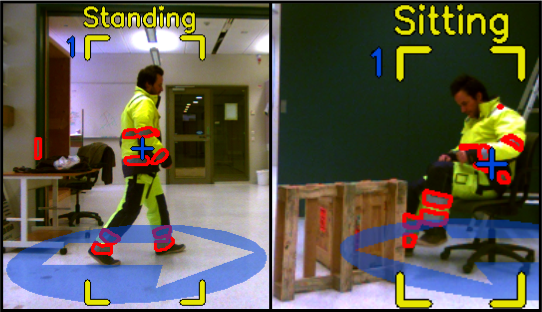
\includegraphics[width =0.99\linewidth]{figs/person_detection}
    % \vspace{-0.25cm}
    \caption{\textit{Human detection:} For safe navigation, the robot detects and tracks humans in
      the close neighborhood, estimates their position, and infers body pose information. Active
      infrared vision in combination with reflective safety clothing ensures robust performance
      independent of the illumination conditions.}
    \label{fig:people_det}
    \vspace{-0.55cm}
  \end{center}
\end{figure}
% 
As the envisioned mobile manipulation system will operate in environments shared with human
workforce, robust human detection is crucial to ensure a safe work environment. We address this
problem by using the recently developed RefleX workforce protection system~\cite{Mosb14}. RefleX is
a camera-based safety system designed for industrial vehicles and machinery, that detects and tracks
human workers wearing off-the-shelf high-visibility clothing (Fig.~\ref{fig:people_det}). Using
active near-infrared stereo vision, RefleX detects and locates the reflective markers on the safety
garments in order to estimate position and relative velocity of the observed person, and to infer
further body pose information. The underlying sensing principle thereby ensures that the detection
performance is nearly independent of external illumination conditions. A classification of the
observed reflective patterns further allows the APPLE system to discriminate between a worker's
safety garments and other reflective navigation markers placed in the environment.

%
\section{Grasping \& Manipulation System}
\label{sec:manip}
%
\hl{Introduce LBR iiwa + Velvet Fingers 2 Gripper setup}
%
\subsection{Related Work}
\label{subsec:Grasping_related_work}
%
 Current autonomous grasping systems~\cite{Bere07, Srin10, Krug14a}
commonly employ sampling based planners~\cite{LaVa06} to generate online reach-to-grasp motion plans
for offline planned grasps which are stored in a database. During the execution phase, such
approaches necessitate many futile motion planning attempts which often incurs significant time
delays mainly due to the frequent colli- sion checks which are necessary to avoid the robot coming
in contact with itself or the environment.  For APPLE, we adopted a real-time reactive control
approach for manipulator mo- tion generation which allows to exploit redundancy, opposed to the
commonly used sense-plan-act architectures which constrain all manipulator DoF. The main idea is to
formulate a hierarchical set of tasks~\cite{Sams91} such as “move end-effector on this plane” or
“avoid joint limits” and to compute controls such that tasks of lower priorities are exe- cuted in
the null-space of higher ranked tasks~\cite{Sici91, Sent10}.

The aim is to reduce the dependence on classical, sampling based motion planning and to move towards
reactive feedback control to generate and execute complex motion behaviors of a robot.  Here, only
high-level behavioral goals (e. g., “go to this region” or “stay above obstacle plane”) are
specified in form of task functions~\cite{Sams91}. An intelligent control algorithm, which is based
on embedded optimization of these task functions, then handles the details and synthesizes
appropriate motions automatically in an online fashion. Opposed to classical sense-plan-act
architectures, in this paradigm only task-relevant Degrees of Freedom (DoF) need to be constrained,
which allows to exploit kinematic redundancies, e. g., for a manipulator to avoid unexpected
obstacles. Regarding grasp planning, we follow the general tenet and will extract redundant
representations in form of constrained pose intervals instead of discrete poses
%
\subsection{Object Detection}
Typical commissioning scenarios in a warehouse environment would generally involve as a first step the identification and localization of an object targeted for picking.
There are however many application scenario specific factors to consider when designing an object detection system for this task. 
For example: a single pallet may hold a homogeneous or a heterogeneous set of objects; objects may be stored in boxes and equipped with barcodes; objects may be stored on shelves, pallets, or simply piled up.
For the APPLE project we assumed a simple scenario where objects of the same type are stored on a single pallet.
We have equipped the Velvet Fingers 2 gripper with a structured light depth sensor: the Structure IO\footnote{\url{http://structure.io/}} device. 
We use the 3D point clouds generated by the sensor as an input for a simple object detection module which identifies clusters of points matching our expected object models.
The object detection module was implemented using the point cloud library (PCL)\footnote{\url{http://pointclouds.org/}} following the simple algorithm described in Alg.~\ref{alg:obj}.
%
\begin{algorithm}[tbh]
%\DontPrintSemicolon
\SetKwInOut{Input}{input}
\SetKwInOut{Output}{output}
\Input{Pointcloud $P$, kinematic model $K$, joint positions $\mbm{j}$}
\Output{Target cluster $T$}
Transform $P$ into world coordinates using $K,\mbm{j}$\;
\While {target plane not found} {
    Extract plane $\mbm{n},d$ from $P$ using RANSAC\;
    \If{$\mbm{n}\mbm{z} < \cos{\alpha}, abs(d-h_{pallet}) < e_{pallet}$}{target plane found\;}
    \Else{ Remove inliers and iterate. If points in $P$ less than $20\%$ of original points, report failure\;}
}
Extract oriented bounding box (OBB) of plane inliers\;
Extract points inside OBB and height in $(d,d+d_{eps})$\;
Euclidean cluster points in $P_n$\;
\For{each cluster $E_i$} {
    Fit a ML Gaussian to $E_i$ as $\mu_i,\Sigma_i$\;
    Eigen decomposition $\Sigma_i=Q\Lambda Q^{-1}$\;
    Let $\mbm{q}_1$ be the eigenvector associated to the largest eigenvalue $\lambda_1$\;
    \If{$\mbm{q}_1\mbm{z} < \cos{\alpha}$ and $\lambda_2 < r_{max}$} {report target cluster at $\mu_i,\Sigma_i$\;}
}
\caption{Object detection algorithm}\label{alg:obj}
\end{algorithm}
%
\par
The basic idea of Alg.~\ref{alg:obj} is to first detect the location of the pallet plane, then to extract the points belonging to objects on the pallet, cluster them and then analyze the obtained clusters. The parameters in this algorithm are: $h_{pallet}$ --- the expected height of the pallet above floor level; $e_{pallet}$ --- a tolerance of the pallet height; $\alpha$ --- a tolerance on the angle that the pallet plane normal makes with the vertical axis $\mbm{z}$; $r_{max}$ --- the maximum radius of a graspable cylinder. Each of the detected clusters is analyzed using PCA, checking that the dominant point distribution is along the $\mbm{z}$ axis and that the $x-y$ point spread is within the graspable objects limit. Identified target clusters are then passed on to the grasp planning module.
\subsection{Grasp Planning}
\begin{figure*}[t!] 
   \centering
    %\def\svgwidth{200pt} 
    \input{figs/grasp_interval.pdf_tex} 
   \caption{\textit{Grasp interval:} (Left) todo ... (Right) truncated grasp interval ...} 
   \label{fig:grasp_interval}
\end{figure*}
%\FloatBarrier
%

\cite{Bohg14}(data driven grasping) (SotA autonomous grasping systems) \cite{Pas13} cylinder shell
fitting

The key challenge for many applications of robotic mobile manipulation is autonomous grasping in
uncertain real-world environments. Finding collision-free trajec- tories leading the gripper-arm
chain from a given initial to a reachable final state (grasp planning together with vehicle and
manipulator motion planning) constitutes the fundament for any robot manipulation system. Currently,
despite of a large research effort, no commercially viable solution is available for this
problem. In today’s state-of-the-art autonomous grasping systems~\cite{Bere07, Srin10, Krug14a},
grasp planning and motion planning are usually seen as independent sub-problems~\cite{Dian10}. A
database storing object models together with pre-computed grasps is used to relax the need to find
suitable gripper poses/configurations~\cite{Mill04, Gold11, Krug14a}. In the online stage, sampling
based planners~\cite{LaVa06} attempt to generate valid trajectories for the pre-planned grasps,
which are executed in a feasible-first manner~\cite{Bere07}. During the execution phase, such
approaches necessitate many futile motion planning attempts, which often incurs significant time
delays since sampling based planners suffer from the curse of dimensionality. Also, while being able
to solve complicated planning problems if given enough time, these planners don’t scale well to
geometrically simple scenarios~\cite{Ratl09} and they are ill suited to incorporate contact events
with the environment.

 Instead of representing grasps as discrete gripper wrist poses and joint
configurations, we use grasp interval regions as depicted in Fig.~\ref{fig:grasp_interval}. These
grasp intervals can easily be transcribed as target tasks for the manipulator motion control and
allow for redundancy in the manipulator wrist positioning which eases reach-to-grasp
acquisition. Grasp interval formulation depends on the specific target object and has to be verified
experimentally. For now, we constrain ourselves to cylindrical objects as shown in
Fig.~\ref{fig:grasp_interval}. We then rely on the inherent capabilities of the grasping device and
the compliance of the system for successful grasp execution as stated below.


\cite{Bala12}(Identifying grasp principles from humans) \cite{Gien08a, Gien08b, Vahr10}(Task maps with RRT)
%
\subsection{Manipulator Motion Generation}
\label{subsec:manip_motion}
%
 \cite{Sams91}(task functions)
~\cite{Sici91, Sent10}(Redundant motion generation)

We lean on the notation in~\cite{Esca14} and define the manipulator joint configuration by the
vector $\mbm{q}$ and the control inputs as corresponding joint velocities $\dot{\mbm{q}}$. A task
function is any derivable function of $\mbm{e}$. To give an example, a task with the purpose of
bringing an end-effector point $\mbm{p}(\mbm{q})$ onto a plane described by unit normal $\mbm{n}$
and offset $b$ can be transcribed by the task function $\mbm{e}=\mbm{n}^T\mbm{p}(\mbm{q})-d$, which
formulates the projection residual between the plane and $\mbm{p}(\mbm{q})$ \hl{connect example to
  the previously described grasp interval}. The task evolution is given by
$\mbm{J}\dot{\mbm{q}}=\dot{\mbm{e}}$ with task jacobian
$\mbm{J}=\frac{\partial\mbm{e}}{\partial\mbm{q}}$.

Goal is to compute joint velocities such that the task evolution follows a desired reference profile
$\dot{\mbm{e}}^*$ (often chosen as exponential decay $\mbm{e}^*= -\lambda \mbm{e}$, with $\lambda
\in \mathbb{R}_+$). For a single equality task, this necessitates to solve the following least
squares Quadratic Program (QP)
%
\begin{align}\label{eq:QP}
  \dot{q}^* &\in \mbox{arg} \; \underset{\footnotesize\dot{\mbm{q}}\normalsize}{\mbox{min}}||\mbm{J}\dot{\mbm{q}}-\dot{\mbm{e}}^*||.
\end{align}
%
In order to allow for inequality tasks, we henceforth use a general task formulation with upper
bounds 
\begin{align}\label{eq:task}
 \mbm{J}\dot{\mbm{q}}&\leq \mbm{e}^*
\end{align}
%
as in~\cite{Esca14}. This allows to transcribe lower bounds $\mbm{J}\dot{\mbm{q} \geq \mbm{e}^*}$,
double bounds $\dot{\underline{\mbm{e}}}^* \leq \mbm{J}\dot{\mbm{q} \leq \dot{\bar{\mbm{e}}}^*}$ and
equalities $\mbm{J}\dot{\mbm{q}=\mbm{e}^*}$ by reformulating the task respectively as
$-\mbm{J}\dot{\mbm{q} \leq -\mbm{e}^*}$, $\begin{bmatrix} -\mbm{J} \\
  \mbm{J} \end{bmatrix}\dot{\mbm{q}} \leq \begin{bmatrix} -\dot{\underline{\mbm{e}}}^*
  \\ \dot{\bar{\mbm{e}}}^* \end{bmatrix}$ and $\begin{bmatrix} -\mbm{J} \\
  \mbm{J} \end{bmatrix}\dot{\mbm{q}} \leq \begin{bmatrix} -\dot{\mbm{e}}^* \\
  \dot{\mbm{e}}^* \end{bmatrix}$.

If the constraint $\mbm{J}\dot{\mbm{q} \leq \mbm{e}^*}$ is infeasible, a least squares solution for
$\mbm{q}^*$ as in~\eqref{eq:QP} can be found by introducing the slack variable $\mbm{w}$ in the
decision variables
%
\begin{align}\label{eq:iQP}
  &\underset{\dot{\mbm{q}},\;\mbm{w}}{\mbox{min}}\;\;||\mbm{w}||\\
   \mbox{subject to} \quad &\mbm{J}\dot{\mbm{q}} \geq \mbm{e}^* + \mbm{w}. \nonumber
\end{align}
%
To form a stack of hierarchical tasks with $p=1,\dots,P$ priority levels, we stack all task
jacobians in~\eqref{eq:task} with the same assigned priority in a matrix $\mbm{A}_p$, and all
corresponding reference velocities in a vector $\mbm{b}_p$ to form a constraint of the form
$\mbm{A}_p\dot{\mbm{q}}\leq \mbm{b}_p$ for each hierarchy level. The aim is to sequentially satisfy
a constraint at best in the least square sense while solving for the subsequent constraint of lower
priority in the null-space of the previous constraint, such that the previous solution is left
unchanged. Therefore, the following QP, where the previous slack variable solutions $\mbm{w}_i^*$
are frozen between iterations, needs to be solved for $p=1,\ldots,P$
%
\begin{align}\label{eq:HiQP}
  &\underset{\dot{\mbm{q}},\;\mbm{w}_p}{\mbox{min}}\;\;||\mbm{w}_p||\\
   \mbox{subject to} \quad &\mbm{A}_i\dot{\mbm{q}} \leq \mbm{b}_i + \mbm{w}_i^*, \quad i=1,\dots,p-1 \nonumber \\
                           &\mbm{A}_p\dot{\mbm{q}} \leq \mbm{b}_p + \mbm{w}_p.  \nonumber 
\end{align}
%
The final joint velocity vector $\mbm{q}^*$ is obtain from the $P^{\mbox{th}}$ solution
of~\eqref{eq:HiQP}.

For reactive on-the-fly motion generation we formulate a stack of hierarchical tasks and use the
recently developed method by Kanoun et al.~\cite{Kano11}, which allows to account for inequality
tasks and solves a sequence of convex optimization problems at each time step to obtain
appropriate joint velocity commands (the method also can be used to directly generate torque
commands while accounting for the robot dynamics~\cite{Saab13}).
 
Obstacle avoidance is also achieved on a control-level, by formulating tasks which maintain minimum
distances between simple geometric primitives such as spheres, planes, points and capsules. We argue
that for the considered application strict collision avoidance is neither necessary nor desired,
since picking and manipulation inherently necessitates contact events between the robot and the
environment. Also, in real-world applications where knowledge about the environment is available
only in form of noisy sensor data, it might not be possible to avoid contacting the environment
without being overly conservative. This makes the KUKA LBR iiwa with its compliant low-level control
schemes and contact detection abilities an ideal platform for the tackled purpose and motion
generation scheme. The relatively simple picking task in APPLE provides an ideal testbed in a
real-world scenario.

\cite{Kano09}(Task function descriptions)
%
\subsection{Robust Grasp Execution}
\label{subsec:grasp_execution}
%


\begin{figure}[!t]
 \centering
   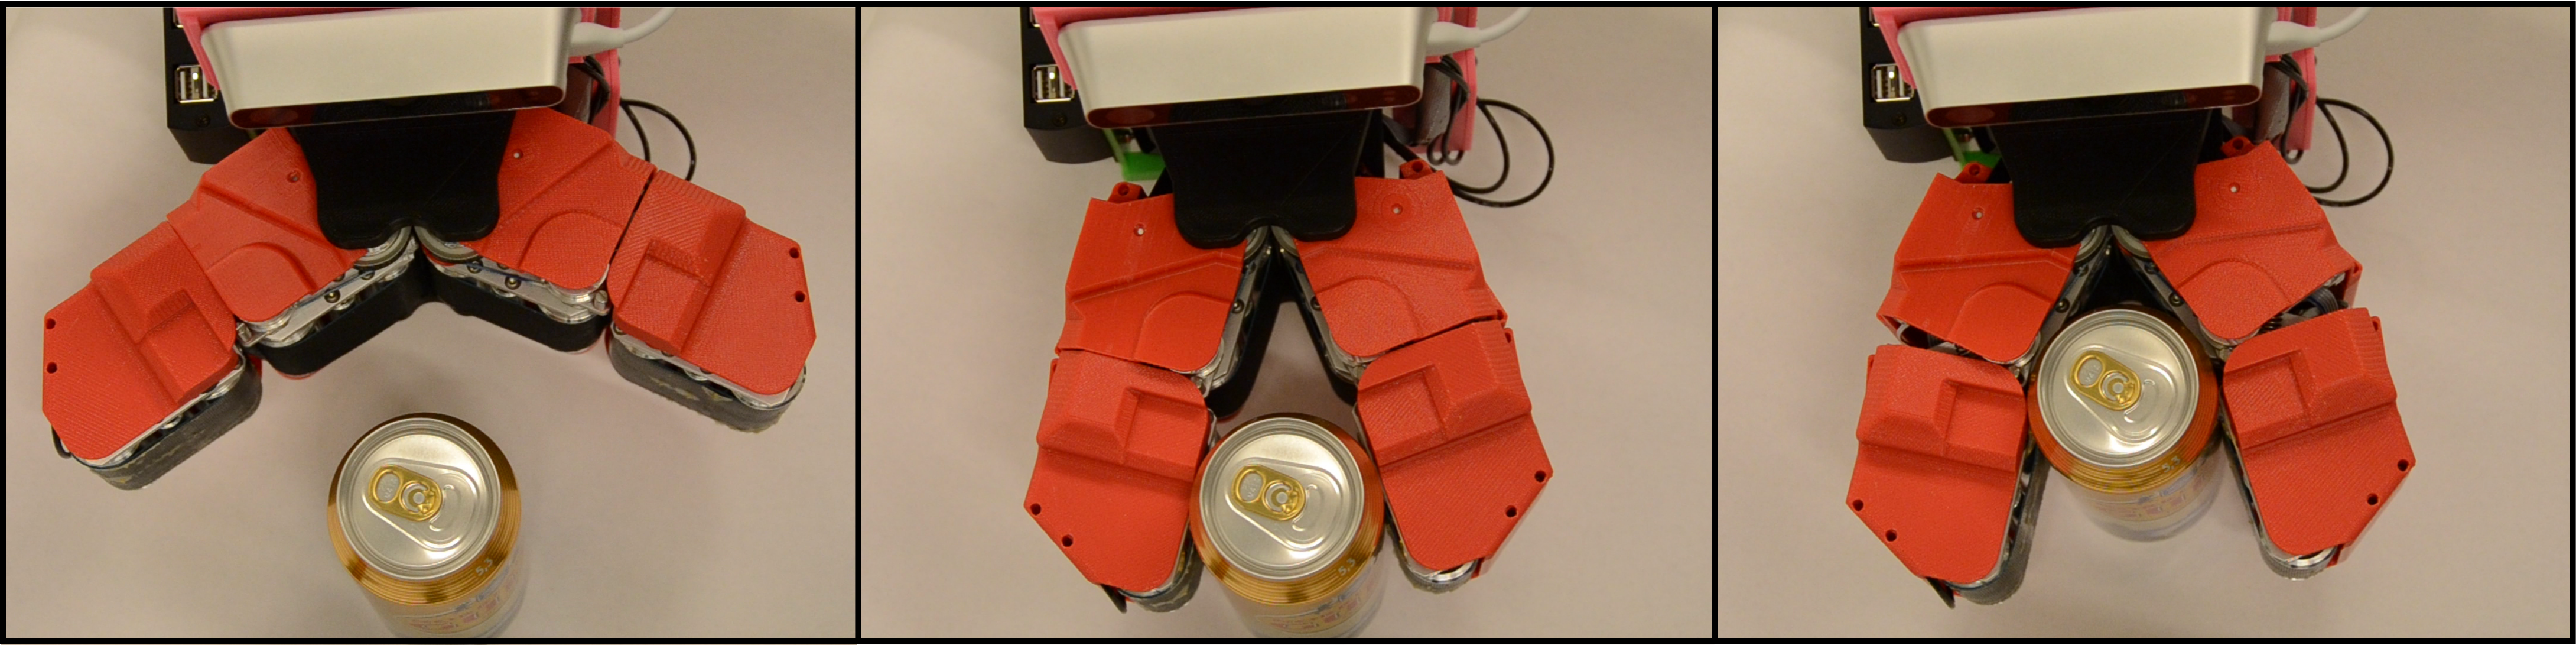
\includegraphics[width = 1.0\linewidth]{figs/pull_in}
   \caption{\textit{Pull-in grasping strategy:} Depicted is a sequence of intermediate grasp states
     where the belts of the gripper are used to pull the object towards its palm which results in a
     transition from a fingertip to an enveloping grasp.}
   \vspace{-4mm}
   \label{fig:pull_in}
   \centering
 \end{figure}
%
\begin{figure*}[!t]
 \centering
   \subfigure[]{\includegraphics[width = .32\linewidth]{figs/vcg1}}
   \subfigure[]{\includegraphics[width = .32\linewidth]{figs/vcg2}}
   \subfigure[]{\includegraphics[width = .32\linewidth]{figs/vcg3}}
   \caption{\textit{Grasp Execution Control:} As the open griper closes in on the object (Left), the
     current through the opening motor is monitored. When contact is made (Middle), the actuated
     belts are switched on to pull in the object. The controller then strives to maintain the
     current in between two target thresholds by opening or closing the gripper during in-hand
     manipulation (Right).}
   \label{fig:pull_in_control}
 \centering
\end{figure*}
%
For this component, we leverage the capabilities of the Velvet Gripper, namely underactuation and
conveyor belts on the finger pads in order to achieve robust grasping behavior. Especially in
cluttered scenes, a ``pull-in'' strategy has been shown to be especially effective to achieve stable
grasps while starting from a relatively wide range of initial gripper poses with respect to the
target object~\cite{Krug14a}. Here, the features of the grasping device are exploited to embrace the
object in a firm envelope grasp by simultaneously squeezing it in a compliant fashion while
actuating the belts inwards.

(\hl{the following is copy/pasted from the Gripper control workshop paper})~\cite{Krug14c} Each of
the gripper’s two fingers has a planar manipulator structure with two joints and active surfaces
which are implemented by coupled conveyor belts on the inside of the two phalanges. The mechanical
structure is underactuated and comprises only one actuated Degree of Freedom (DoF) for opening and
closing and two DoF for the belt movements.  If, during grasping, the proximal phalanges are blocked
by an object, the gripper’s distal phalanges continue to “wrap around” and envelope it in a firm
grasp.  The experiments reported in~\cite{Krug14a} showed, that in cluttered scenes fingertip
grasps are more likely to be feasible than robust enveloping grasps, because the latter necessitate
large opening angles resulting in bulky gripper silhouettes for which no collision free approach
trajectories can be found. Therefore, we employ the “pull-in” strategy which is illustrated in
Fig.~\ref{nothereyet}. Here, the underactuated nature and the conveyor belts on the grasping device
are exploited to embrace the object in a firm envelope grasp by simultaneously squeezing it while
actuating the belts inwards. This is achieved by compliant low-level position controllers which
saturate on experimentally evaluated current thresholds. We use a simple grasping routine which is
triggered after an initial fingertip grasp is achieved (see Fig.~\ref{nothereyet}). This routine
consists of issuing commands to fully close the gripper while moving the belts a pre-defined offset
towards the palm. Three thresholds on the current absorption of the opening motor are used: a low
threshold (LT) signifies contact between the gripper and the object and a mid threshold (MT)
indicates a large enough contact force to stop the closing movement.  Finally, an upper threshold
(UT) prevents damage to the grasping device. Once the pull-in sequence is completed, the controllers
maintain the final torques to ensure a stable grasp.


%
\section{Evaluation}
\label{sec:eval}

\cite{Guro15}(Used off-the-shelf solver)
\cite{Quig09}(ROS)
%
\section{Discussion and Outlook}
\label{sec:discussion}
%
In this paper, we presented a research platform for autonomous picking and palletizing (APPLE) for
fully autonomous commissioning tasks in intralogistics settings. The APPLE robot comprises a
nonholonomic mobile base with the ability to autonomously detect and pick standard EUR half-pallets
from designated loading areas. Also incorporated is a camera system for the detection and avoidance
of human workers wearing reflective safety clothing. The manipulation system for loading/unloading
unstructured goods from pallets operates on a novel redundant grasp representation as intervals in
task space, which allows to incorporate empirical knowledge. We leverage the obtained redundancy by
generating reactive manipulator motions on the fly, by using a prioritized control approach which
allows to formulate the target object picking as a stack of hierarchical tasks~\cite{Kano11}. Also,
we provide an early experimental evaluation of the APPLE system by means of successfully executed
trials of a simplified commissioning task (see the video attachment).

The presented work is limited to the picking of objects with cylindrical shapes, future work will
aim at extending our grasp interval representation to other primitive shape types. Also, we work on
a computational method to parametrize the interval for a current scene which, right now, is done
empirically. 


%\cite{Tass12}\cite{Kuma13}(optimal control for motion generation)

%
\section*{Acknowledgments}
%
The authors would like to thank Per Sporrong, Bo-Lennart Silfverdal, Bengt {\AA}sberg and Joakim
Larsson at {\"O}rebro University for their engineering support.
%
\bibliographystyle{IEEEtran}
\bibliography{References}

% \newpage
% REMARKS:
% \begin{itemize}
% \item cite the books stating that shifting of initial states is not a problem
% \end{itemize}

\end{document}



